
This chapter describes the work done in each sprint. A sprint is one iteration of the Scrum process
(see section \ref{section:scrum} for more information about Scrum). The duration of each sprint is two weeks.
Every sprint gets assigned various tasks from the backlog and each task is given a specific point value.
This point value is an abstract estimation of the amount of work that is required to finish the task.
The point value can be also influenced by the importance of the task. If a task requires more time than
planned and is not finished by the end of the sprint, it will be assigned a 'prolonged' status and
moved to the next sprint.

\newpage

\section{First sprint}

Duration: 20/01 to 02/02
Points total: 92

The first sprint was dedicated to planning meetings and working hours
and studying about interested technologies. The team also did a lot of
brainstorming in order to identify possible product ideas to show the
customer and produced some small proof of concept applications.

\begin{table}[ht!]
\begin{tabular}{ | l | c | r | }

\hline
\textbf{Task} & \textbf{Points} & \textbf{Status} \\
\hline

Exchange contact information		& 1  & done \\
\hline
Plan group meetings			& 2  & done \\
\hline
Meet with the customer			& 4  & done \\
\hline
Plan meetings with the customer		& 2  & done \\
\hline
Brainstorm ideas about the product	& 18 & done \\
\hline
Search for similar products		& 14 & done \\
\hline
Proof-of-concept application		& 12 & done \\
\hline
Read on development processes		& 4  & done \\
\hline
Choose a development process		& 6  & done \\
\hline
Read Facebook developers' pages		& 8  & done \\
\hline
Read on OpenSocial			& 10 & done \\
\hline
Read on Arduino				& 8  & done \\
\hline
Setup mailing list			& 1  & done \\
\hline
Setup a skype chat			& 1  & done \\
\hline
Setup a GIT repository			& 1  & done \\
\hline

\end{tabular}
\end{table}

\begin{figure}[h!]
\centering 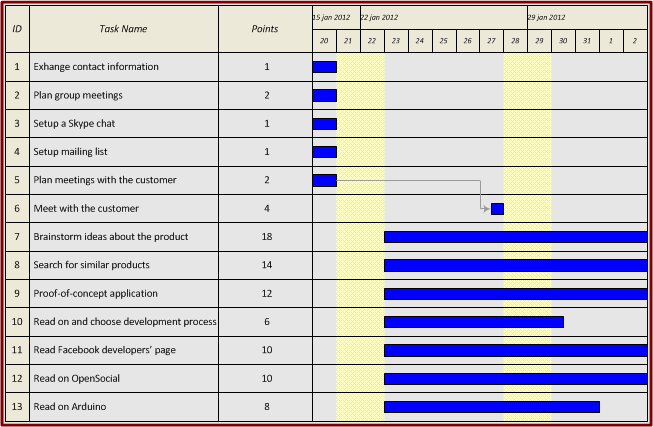
\includegraphics[scale=0.8]{img/sprints-gantt1.png}
\caption{Gantt diagram for the first sprint}
\label{fig:sprints-gantt1}
\end{figure}

\newpage


\section{Second sprint}

Duration: 03.02 to 16.02
Points total: 99

The second iteration was focused on producing more prototypes of the product to
show the customer in order to receive the necessary feedback to identify
the product requirements and begin designing the different parts of the system,
as well as acquiring necessary knowledge and confidence with the involved
technologies. The team also worked on the preliminary version of the report.
The customer told us that in order to show the re-usability capabilities of
our code we needed to produce two more prototypes, which can be considerably
simpler than the t-shirt prototype.

\begin{table}[ht!]
\begin{tabular}{ | l | c | r | }

\hline
\textbf{Task} & \textbf{Points} & \textbf{Status} \\
\hline

Present a working prototype	(Week 1)	& 18 & done \\
\hline
Delivery of preliminary report			& 24 & done \\
\hline
Present a working prototype	(Week 2)	& 8  & done \\
\hline
Estabilish a bluetooth connection to Arduino	& 8  & done \\
\hline
Estabilish a connection to Facebook
(using Facebook's SDK)				& 6  & done \\
\hline
Study Android applicationd development		& 10 & done \\
\hline
Study Facebook Android SDK			& 12 & done \\
\hline
Study Android SDK				& 12 & done \\
\hline
Setup ScrumDo					& 1  & done \\
\hline

\end{tabular}
\end{table}

\begin{figure}[h!]
\centering 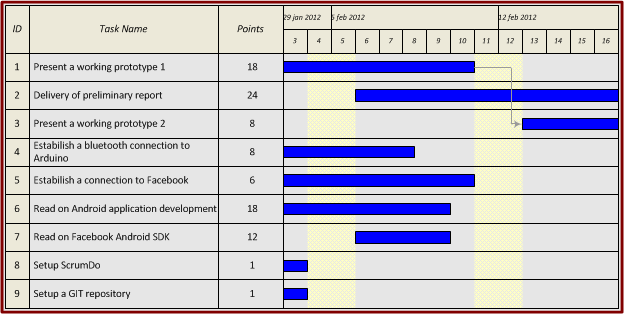
\includegraphics[scale=0.8]{img/sprints-gantt2.png}
\caption{Gantt diagram for the second sprint}
\label{fig:sprints-gantt2}
\end{figure}

\newpage

\section{Third sprint}

Duration: 17.02 to 01.03
Points total: 108

This sprint was focused on proceeding with the design based on the
feedback received from the customer. An initial version of the Communication
library was also designed and coded. Design of the Social library also began.
We delivered a list of hardware we needed to build our t-shirt prototype.

\begin{table}[ht!]
\begin{tabular}{ | l | c | r | }

\hline
\textbf{Task} & \textbf{Points} & \textbf{Status} \\
\hline

Present a working prototype (Week 1)		& 18 & done \\
\hline
Present a working prototype (Week 2)		& 8  & done \\
\hline
Initial system design				& 14 & done \\
\hline
Social library design (part I)			& 20 & done \\
\hline
Communication library design (part I)		& 20 & done \\
\hline
Communication library coding (part I) 		& 16 & done \\
\hline
Read on Android IPC mechanisms			& 12 & done \\
\hline

\end{tabular}
\end{table}

\begin{figure}[h!]
\centering 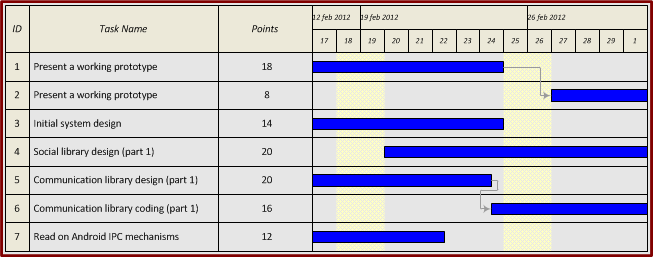
\includegraphics[scale=0.8]{img/sprints-gantt3.png}
\caption{Gantt diagram for the third sprint}
\label{fig:sprints-gantt3}
\end{figure}

\newpage


\section{Fourth sprint}

Duration: 02.03 to 15.03
Points total: 112

This sprint was mainly aimed to the delivery of the mid-term report as well
as polishing of the Communication library. The system design was revised in
order to suit the customer requirements. The design of the Social library couldn't
be completed in time due to design issues. These issues were presented to the
customer who provided valuable feedback that helped solve them.
We will hopefully receive our hardware in the next weeks, before Easter vacation.

\begin{table}[ht!]
\begin{tabular}{ | l | c | r | }

\hline
\textbf{Task} & \textbf{Points} & \textbf{Status} \\
\hline

Work on the report			& 24 & done \\
\hline
Present a working prototype		& 18 & done \\
\hline
System design				& 18 & done \\
\hline
Social libray design (part II)		& 14 & prolonged \\
\hline
Social library coding (part I)		& 10 & done \\
\hline
Comm. library design (part II)		& 12 & done \\
\hline
Comm. library coding (part II)		& 16 & done \\
\hline

\end{tabular}
\end{table}

\begin{figure}[h!]
\centering 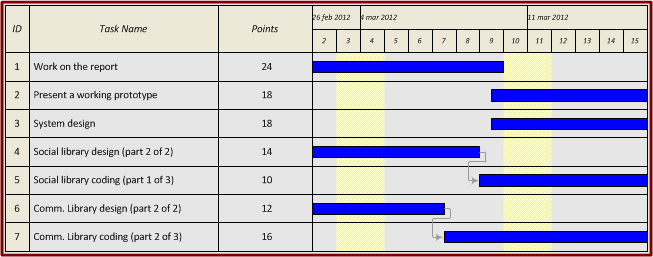
\includegraphics[scale=0.8]{img/sprints-gantt4.png}
\caption{Gantt diagram for the fourth sprint}
\label{fig:sprints-gantt4}
\end{figure}

\newpage

\section{Fifth sprint}

Duration: 16.03 to 29.03
Points total: 128

During this sprint the team produced yet another prototype for the customer
and proceeded with the design and coding of the Social library.
Coding of the Communication library also continued, and an initial version
was deployed by the end of the sprint. The team also did some brainstorming
and identified the other two prototypes that were to be presented together with
the T-Shirt prototype. Some proof-of-concept applications for these
prototypes were also made. This sprint was a bit more intense than the previous
ones to cope with the fact that the next sprint would have coincided with Easter vacation.
We still didn't receive the hardware we need in order to begin building the t-shirt
prototype.

\begin{table}[ht!]
\begin{tabular}{ | l | c | r | }

\hline
\textbf{Task} & \textbf{Points} & \textbf{Status} \\
\hline

Present a working prototype		& 18 & done \\
\hline
Social library design (part II)		& 24 & completed \\
\hline
Social library coding (part II)		& 20 & done \\
\hline
Communication library coding (Part III)	& 22 & done \\
\hline
Deploy the Comm. library		& 14 & done \\
\hline
Temperature Prototype research		& 6  & done \\
\hline
Temperature prototype coding (I)	& 10 & done \\
\hline
Led prototype research			& 4  & done \\
\hline
Led prototype coding			& 10 & done \\
\hline

\end{tabular}
\end{table}


\begin{figure}[h!]
\centering 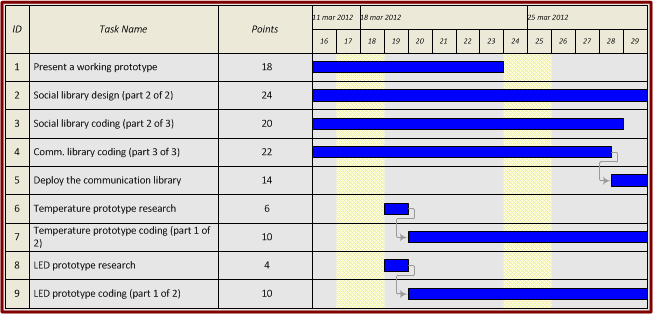
\includegraphics[scale=0.8]{img/sprints-gantt5.png}
\caption{Gantt diagram for the fifth sprint}
\label{fig:sprints-gantt5}
\end{figure}


\newpage

\section{Sixth sprint}

Duration: 30.03 to 12.04
Points total: 50

As this sprint coincided with Easter vacation, little
was planned for this sprint except some early work on the report
and some coding for the Social library and the second prototype.
During this sprint no meetings with the customer were arranged.
We had a brief, sort of 'unplanned' meeting where we were told
that our hardware hadn't yet been ordered.

\begin{table}[ht!]
\begin{tabular}{ | l | c | r | }

\hline
\textbf{Task} & \textbf{Points} & \textbf{Status} \\
\hline

Work on the report			& 18 & done \\
\hline
Social library coding (part III)	& 16 & done \\
\hline
Temperature prototype coding (II)	& 16 & done \\
\hline

\end{tabular}
\end{table}

\begin{figure}[h!]
\centering 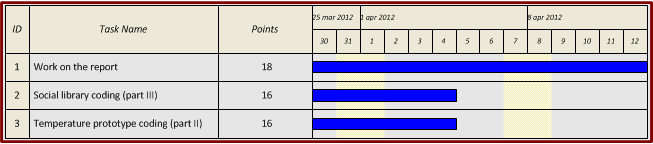
\includegraphics[scale=0.8]{img/sprints-gantt6.png}
\caption{Gantt diagram for the sixth sprint}
\label{fig:sprints-gantt6}
\end{figure}

%\begin{figure}[h!]
%\centering 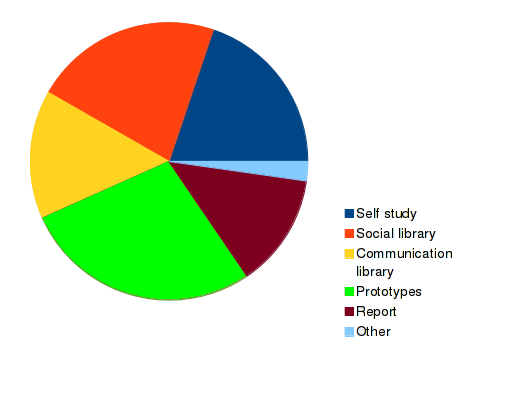
\includegraphics[scale=0.8]{img/sprints-points.png}
%\caption{Story points breakdown}
%\label{fig:sprints-points}
%\end{figure}

\begin{figure}[h!]
\centering 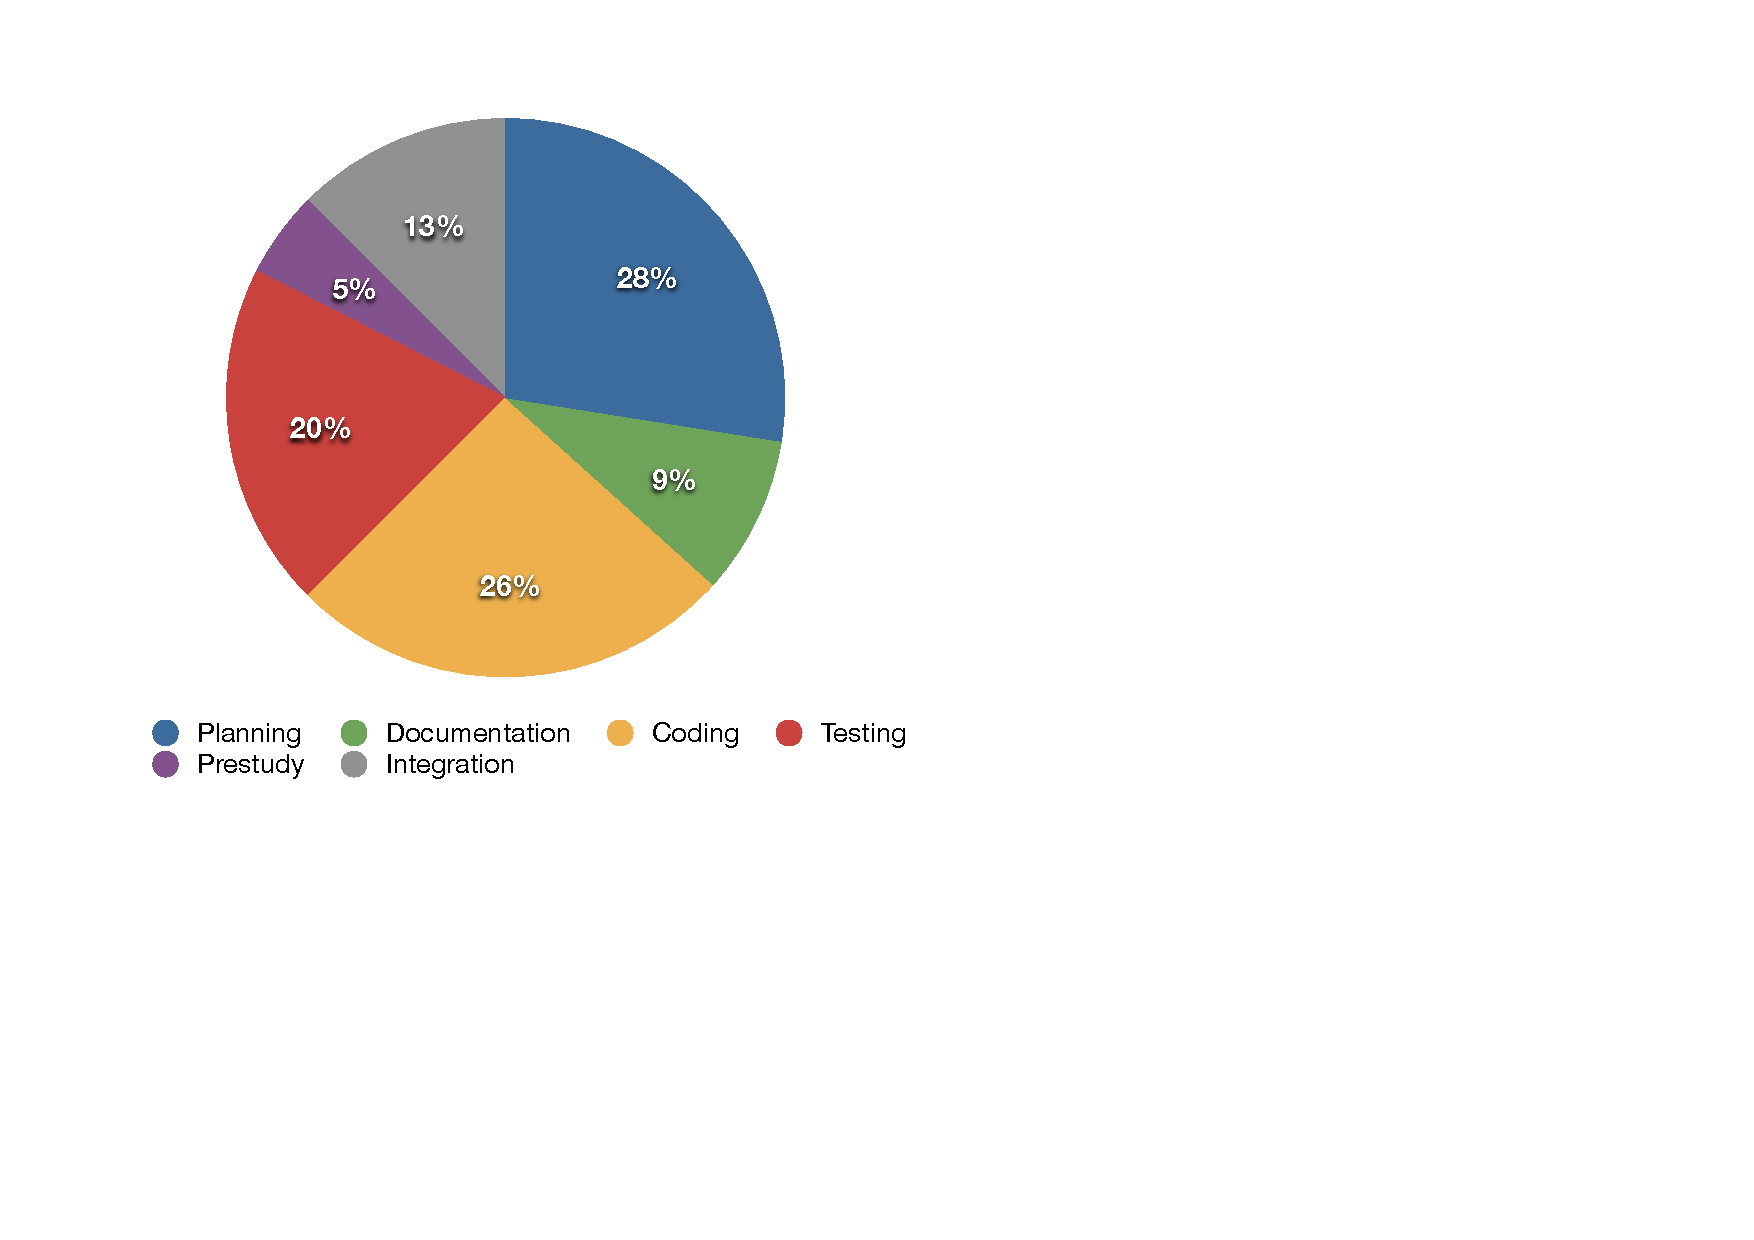
\includegraphics[scale=0.8]{img/pie_chart.pdf}
\caption{Story points breakdown}
\label{fig:sprints-points}
\end{figure}